\chapter{Plasticidade Neural, Aprendizado e Memória}\label{ch:b3:learning-memory}

Em 1953 um cirurgião removeu a parte interna dos dois lobos temporais de
um jovem com epilepsia intratável. As crises diminuíram; o paciente,
conhecido por cinquenta anos como H.M., nunca mais formou uma memória
duradoura de um acontecimento. Ele conseguia manter uma conversa,
aprender a traçar uma estrela num espelho tão bem quanto qualquer um ---
e negar, a cada dia, jamais ter visto a tarefa --- e lembrava-se da
infância. A memória, veio a se descobrir, não era uma coisa só, e a
formação de novas memórias de acontecimentos dependia de uma estrutura
do tamanho de um polegar. O que muda num encéfalo quando ele aprende é a
mais antiga pergunta da neurociência, e sua resposta, elaborada numa
lesma marinha de vinte mil neurônios e em fatias de \omterm{def:b3:learning-memory:kinds}{hipocampo} de rato, é
que as sinapses mudam sua força conforme o que passa por elas --- uma
regra que Donald Hebb adivinhou em 1949 e que uma molécula, o \omterm{prop:b3:learning-memory:nmda}{receptor
NMDA}, acabou por implementar. Este capítulo trata dessa regra e de sua
maquinaria, dos circuitos que a usam para armazenar lugares e
acontecimentos, da matemática que diz o que um sistema desses pode
aprender e quanto pode guardar, e do sinal de recompensa que lhe diz o
que vale a pena aprender.

\section{Tipos de memória e onde eles moram}

\begin{definition}[Formas de aprendizado e de memória]\label{def:b3:learning-memory:kinds}
\index{habituação}\index{sensibilização}\index{condicionamento}\index{memória declarativa}\index{memória procedimental}\index{consolidação}\index{hipocampo}
O aprendizado mais simples é o \emph{não associativo}: a
\emph{habituação}, uma resposta que declina a um estímulo inofensivo
repetido, e a \emph{sensibilização}, uma resposta reforçada depois de um
estímulo nocivo. O aprendizado \emph{associativo} liga dois
acontecimentos: no \emph{condicionamento clássico} (Pavlov) um estímulo
neutro que prevê uma recompensa ou uma punição passa a provocar a
resposta; no \emph{condicionamento operante} uma ação que é recompensada
é repetida. A memória humana se divide em memória \emph{declarativa}
--- fatos e acontecimentos, evocados conscientemente, dependentes do
\emph{hipocampo} e do lobo temporal medial --- e memória \emph{não
declarativa} --- habilidades e hábitos (estriado, \omterm{def:b3:nervous-systems:plan}{cerebelo}), medo
condicionado (amígdala), priming (córtex) ---, expressa no desempenho
sem recordação. Uma memória é guardada primeiro numa forma lábil de
curto prazo, que dura de segundos a horas, e é \emph{consolidada} ao
longo de horas a anos numa forma estável de longo prazo, que já não
precisa do hipocampo e reside no córtex.
\end{definition}

\begin{proof}[Evidência]
Scoville e Milner (1957) relataram o caso de H.M.: depois da remoção dos
dois \omterm{def:b3:learning-memory:kinds}{hipocampos} e do córtex vizinho, sua inteligência e suas memórias
anteriores à operação estavam em grande parte intactas, sua memória de
trabalho era normal enquanto ele prestasse atenção em algo, mas ele não
conseguia formar nenhuma memória nova de um acontecimento ou de um fato.
Ele aprendia habilidades motoras em ritmo normal ao longo de dias,
negando ter praticado --- de modo que a memória de habilidades não
precisava do \omterm{def:b3:learning-memory:kinds}{hipocampo} --- e lembrava melhor o passado remoto que os
anos imediatamente anteriores à cirurgia, de modo que o \omterm{def:b3:learning-memory:kinds}{hipocampo} era
necessário para registrar e, por um tempo, para guardar \omterm{def:b3:learning-memory:kinds}{memórias
declarativas}, mas não para armazená-las para sempre. Macacos e ratos com
lesões equivalentes mostraram a mesma dissociação, e o estudo de um
único paciente reorganizou o campo.
\end{proof}

\section{A regra de Hebb e sua molécula}

\begin{definition}[Plasticidade hebbiana, LTP e LTD]\label{def:b3:learning-memory:ltp}
\index{regra de Hebb}\index{potenciação de longa duração}\index{depressão de longa duração}\index{plasticidade dependente do tempo de disparo}
Hebb (1949) propôs que, quando um neurônio pré-sináptico participa
repetidamente do disparo de um pós-sináptico, a conexão entre eles é
fortalecida --- ``células que disparam juntas conectam-se''. A
\emph{potenciação de longa duração} (LTP) é sua forma experimental: uma
salva breve de estimulação em alta frequência de uma via deixa as
sinapses que ela ativou mais fortes por horas numa fatia e por semanas
num animal. A LTP é \emph{específica da entrada} (só as sinapses
estimuladas mudam), \emph{associativa} (uma entrada fraca pareada com
uma forte para a mesma célula é potenciada) e exige
\emph{\omterm{def:b3:structural-biology:allostery}{cooperatividade}} entre as entradas para despolarizar a célula. A
\emph{depressão de longa duração} (LTD) é seu oposto, produzida por
atividade prolongada em baixa frequência. Na \emph{plasticidade
dependente do tempo de disparo}, o sinal é dado pela ordem: um disparo
pré-sináptico alguns milissegundos \emph{antes} do pós-sináptico
fortalece a sinapse; um logo \emph{depois} a enfraquece, dentro de uma
janela de cerca de \qty{20}{ms} para cada lado --- de modo que uma
sinapse aprende a prever, e não apenas a correlacionar.
\end{definition}

\begin{proposition}[O receptor NMDA como detector de coincidências]\label{prop:b3:learning-memory:nmda}
\index{receptor NMDA}\index{receptor AMPA}\index{CaMKII}\index{CREB}\index{espinha dendrítica}
Nas sinapses excitatórias o glutamato age sobre dois receptores. O
receptor \emph{AMPA} abre ao ligar e conduz a corrente sináptica comum.
O receptor \emph{NMDA} liga glutamato, mas fica bloqueado no potencial
de repouso por um íon de magnésio em seu poro; só quando a membrana
pós-sináptica está despolarizada --- por muitas entradas ao mesmo tempo
ou por um potencial de ação retropropagado --- é que o magnésio é
expulso e o canal conduz, deixando entrar cálcio. O \omterm{prop:b3:learning-memory:nmda}{receptor NMDA} abre,
portanto, apenas quando a liberação pré-sináptica (glutamato) coincide
com a atividade pós-sináptica (despolarização): é a porta ``e'' de Hebb
numa única proteína. O cálcio que entra numa \emph{\omterm{prop:b3:learning-memory:nmda}{espinha dendrítica}}
ativa a quinase \emph{CaMKII}, que fosforila os \omterm{prop:b3:learning-memory:nmda}{receptores AMPA} e leva
mais deles para a sinapse a partir de uma reserva --- a sinapse fica
mais forte em minutos (LTP inicial). Uma elevação de cálcio grande e
lenta ativa, em vez disso, a fosfatase calcineurina, que retira
\omterm{prop:b3:learning-memory:nmda}{receptores AMPA}: a LTD. A potenciação que dura mais de algumas horas
(LTP tardia) precisa de proteína nova: quinases chegam ao núcleo, o
fator de transcrição \emph{CREB} liga genes, e a espinha cresce e pode
se dividir --- a mesma exigência de expressão gênica que separa a
memória de curto prazo da de longo prazo em todo animal estudado.
\end{proposition}

\begin{proof}[Evidência]
Bliss e L\o mo (1973) estimularam a via perfurante que entra no
\omterm{def:b3:learning-memory:kinds}{hipocampo} de coelho com um trem de pulsos e encontraram a resposta
evocada aumentada por horas depois --- a primeira LTP. Collingridge
(1983) mostrou que um bloqueador do \omterm{prop:b3:learning-memory:nmda}{receptor NMDA} (AP5) impedia a
indução da LTP, mas não a resposta sináptica comum; Morris (1986)
infundiu AP5 no \omterm{def:b3:learning-memory:kinds}{hipocampo} de ratos e verificou que eles já não
conseguiam aprender a posição de uma plataforma escondida numa piscina,
embora nadassem e enxergassem normalmente; e camundongos em que o
\omterm{prop:b3:learning-memory:nmda}{receptor NMDA} foi deletado apenas na região \omterm{def:b3:learning-memory:hippocampus}{CA1} do \omterm{def:b3:learning-memory:kinds}{hipocampo} não tinham
nem LTP ali nem memória espacial. O mesmo receptor, no mesmo lugar, era
necessário para a mudança sináptica e para o aprendizado.
\end{proof}

\begin{omfigure}
\begin{tikzpicture}[every node/.style={font=\scriptsize}, >=stealth]
  % presynaptic terminal
  \draw[thick, omDef, fill=omDef!12] (0,2.2) .. controls (0,3.4) and (4,3.4) .. (4,2.2) -- (4,1.7) -- (0,1.7) -- cycle;
  \node at (2,2.8) {terminal pré-sináptico};
  \foreach \p in {(0.8,2.0),(1.6,2.1),(2.6,2.0),(3.3,2.1)} \draw[thick, fill=omDef!40] \p circle (0.17);
  \foreach \p in {(1.2,1.45),(2.0,1.5),(2.9,1.42)} \fill[omProp] \p circle (0.06);
  \node[right, omProp] at (3.3,1.45) {glutamato};
  % postsynaptic spine
  \draw[thick, omMeth!70!black, fill=omMeth!10] (-0.6,1.1) -- (4.4,1.1) -- (4.4,-1.2) -- (-0.6,-1.2) -- cycle;
  \node at (0.6,-0.9) {espinha dendrítica};
  % AMPA
  \draw[thick, fill=omMeth!45] (0.2,0.85) rectangle (0.6,1.35); \node[below, align=center] at (0.1,0.8) {AMPA:\\entra Na$^{+}$};
  \draw[->, thick] (0.4,1.7) -- (0.4,0.95);
  % NMDA with Mg
  \draw[thick, fill=omThm!35] (2.4,0.85) rectangle (2.9,1.35); \fill[gray!70] (2.65,1.1) circle (0.09); \node[right, font=\tiny] at (2.95,1.1) {bloqueio por Mg$^{2+}$};
  \node[below, align=center] at (2.65,0.8) {NMDA: precisa de glutamato\\\emph{e} de despolarização};
  \draw[->, thick, omThm] (2.65,0.15) -- (2.65,-0.5) node[below] {Ca$^{2+}$};
  % downstream
  \node[draw, rounded corners, fill=omThm!15, font=\tiny] (cam) at (5.6,0.3) {CaMKII};
  \draw[->, thick] (2.9,-0.5) -- (cam);
  \node[draw, rounded corners, fill=omMeth!25, font=\tiny, align=center] (ampa) at (8.2,1.0) {mais receptores AMPA\\inseridos: LTP inicial (minutos)};
  \node[draw, rounded corners, fill=omMeth!25, font=\tiny, align=center] (creb) at (8.2,-0.5) {CREB, proteínas novas,\\crescimento da espinha: LTP tardia (horas+)};
  \draw[->, thick] (cam) -- (ampa.west); \draw[->, thick] (cam) -- (creb.west);
  \node[draw, rounded corners, fill=omDef!15, font=\tiny, align=center] (ltd) at (8.2,-1.8) {Ca$^{2+}$ lento e pequeno: calcineurina,\\AMPA retirados: LTD};
  \draw[->, thick, dashed] (2.9,-0.7) .. controls (4.5,-1.6) .. (ltd.west);
\end{tikzpicture}

{\small O \omterm{prop:b3:learning-memory:nmda}{receptor NMDA} como porta de Hebb. O glutamato sozinho abre os
\omterm{prop:b3:learning-memory:nmda}{receptores AMPA}; o canal NMDA só conduz quando a espinha está também
despolarizada e seu magnésio sai. O cálcio que então entra decide o
futuro da sinapse: uma elevação rápida e grande a fortalece; uma lenta e
pequena a enfraquece.}
\end{omfigure}

\begin{omfigure}
\begin{tikzpicture}
\begin{axis}[
  width=6.6cm, height=5.2cm,
  axis x line=bottom, axis y line=left,
  xmin=-20, xmax=120, ymin=0, ymax=220,
  xlabel={minutos}, ylabel={resposta sináptica (\%)},
  xlabel style={font=\small, at={(axis description cs:0.5,-0.12)}, anchor=north}, ylabel style={font=\small},
  tick label style={font=\scriptsize}, xtick={0,30,60,90,120}, ytick={0,100,200},
  clip=false,
]
\addplot[only marks, mark=*, mark size=1pt, omDef] coordinates {(-18,100) (-15,98) (-12,102) (-9,99) (-6,101) (-3,100) (2,195) (5,180) (8,172) (11,168) (15,165) (20,162) (30,160) (40,158) (50,157) (60,156) (70,156) (80,155) (90,155) (100,154) (110,154) (120,154)};
\addplot[only marks, mark=o, mark size=1pt, gray] coordinates {(-18,100) (-12,101) (-6,99) (2,102) (8,100) (15,101) (30,100) (45,99) (60,101) (75,100) (90,100) (105,101) (120,100)};
\draw[->, thick, omThm] (axis cs:0,215) -- (axis cs:0,200); \node[font=\scriptsize, omThm, anchor=south] at (axis cs:0,216) {tétano};
\node[font=\scriptsize, omDef, anchor=south west] at (axis cs:35,168) {via estimulada: LTP};
\node[font=\scriptsize, gray, anchor=north west] at (axis cs:35,95) {via controle: inalterada};
\end{axis}
\begin{axis}[
  at={(7.6cm,0)}, anchor=south west,
  width=6.6cm, height=5.2cm,
  axis x line=middle, axis y line=middle,
  xmin=-60, xmax=60, ymin=-60, ymax=100,
  xlabel={$t_{\text{pré}} - t_{\text{pós}}$ (ms)}, ylabel={$\Delta w$ (\%)},
  xlabel style={font=\small, at={(axis description cs:0.5,-0.06)}, anchor=north}, ylabel style={font=\small, at={(axis description cs:0.5,1.02)}, anchor=south},
  tick label style={font=\scriptsize}, xtick={-40,-20,20,40}, ytick={-40,40,80},
  clip=false,
]
\addplot[very thick, omMeth!70!black, domain=-60:-0.5, samples=60] {80*exp(x/15)};
\addplot[very thick, omThm, domain=0.5:60, samples=60] {-45*exp(-x/25)};
\node[font=\scriptsize, omMeth!70!black, anchor=south east] at (axis cs:-8,62) {pré antes de pós: LTP};
\node[font=\scriptsize, omThm, anchor=north west] at (axis cs:8,-22) {pós antes de pré: LTD};
\end{axis}
\end{tikzpicture}

{\small À esquerda: a \omterm{def:b3:learning-memory:ltp}{potenciação de longa duração} --- depois de um
tétano breve a resposta da via estimulada permanece aumentada por horas,
enquanto uma via não estimulada para as mesmas células fica inalterada
(especificidade de entrada). À direita: a janela de tempo de disparo ---
a sinapse se fortalece se o disparo pré-sináptico vem na frente e se
enfraquece se vem atrás.}
\end{omfigure}

\begin{theorem}[O que uma sinapse hebbiana aprende]\label{thm:b3:learning-memory:hebb}
\index{aprendizado hebbiano!componente principal}\index{regra de Oja}
Seja um neurônio que recebe entradas $\mathbf{x} = (x_{1},\dots,x_{n})$
por pesos $\mathbf{w}$ e responde linearmente, $y = \mathbf{w}\cdot\mathbf{x}$. A \omterm{def:b3:learning-memory:ltp}{regra de Hebb}, $\Delta\mathbf{w} = \eta\, y\,\mathbf{x}$, dá, em média sobre as entradas,
\[
\langle\Delta\mathbf{w}\rangle = \eta\,C\,\mathbf{w}, \qquad C =
\langle\mathbf{x}\mathbf{x}^{\mathsf{T}}\rangle ,
\]
onde $C$ é a matriz de correlação das entradas. Os pesos crescem sem
limite, e crescem mais depressa ao longo do autovetor de $C$ de maior
autovalor: a sinapse passa a detectar o padrão de entrada mais
frequentemente presente --- o \emph{componente principal} de suas
entradas. Com um termo que penaliza pesos grandes, a \emph{regra de
Oja} $\Delta\mathbf{w} = \eta\, y\,(\mathbf{x} - y\,\mathbf{w})$, o
vetor de pesos converge para esse autovetor normalizado a comprimento
unitário, e o neurônio se torna um detector estável da correlação
dominante naquilo que vê.
\end{theorem}
\begin{proof}
Substituindo $y = \mathbf{w}\cdot\mathbf{x} = \mathbf{x}^{\mathsf{T}}
\mathbf{w}$ na \omterm{def:b3:learning-memory:ltp}{regra de Hebb} obtém-se $\Delta\mathbf{w} = \eta\,\mathbf{x}
\mathbf{x}^{\mathsf{T}}\mathbf{w}$, cuja média sobre as
entradas (com $\mathbf{w}$ variando lentamente) é $\eta C\mathbf{w}$. $C$
é simétrica e semidefinida positiva, de modo que tem autovetores
ortogonais $\mathbf{e}_{k}$ com autovalores $\lambda_{k} \ge 0$;
escrevendo $\mathbf{w} = \sum_{k}
a_{k}\mathbf{e}_{k}$, cada componente
obedece a $\Delta a_{k} = \eta\lambda_{k}
a_{k}$ e cresce como $(1 + \eta\lambda_{k})^{t}$, de modo que o componente ao longo do maior
autovalor passa a dominar a direção de $\mathbf{w}$ enquanto seu
comprimento diverge. A regra de Oja tem média $\eta(C\mathbf{w} -
(\mathbf{w}^{\mathsf{T}}C\mathbf{w})\mathbf{w})$; num ponto fixo,
$C\mathbf{w} = (\mathbf{w}^{\mathsf{T}}C\mathbf{w})\mathbf{w}$, de modo
que $\mathbf{w}$ é um autovetor com $\lambda = \mathbf{w}^{\mathsf{T}}
C\mathbf{w} = \lambda|\mathbf{w}|^{2}$, e daí $|\mathbf{w}| = 1$; o
ponto fixo ao longo do maior autovalor é o estável (uma perturbação em
direção a outro autovetor encolhe, já que o autovalor desse autovetor é
menor), o que aqui se admite.
\end{proof}

\begin{example}[Duas entradas]\label{ex:b3:learning-memory:two-inputs}
Um neurônio recebe duas entradas que costumam estar ativas juntas, de
modo que $C =
\begin{pmatrix} 1 & 0.8 \\ 0.8 & 1\end{pmatrix}$. Os
autovetores são $(1,1)/\sqrt{2}$ com autovalor $1.8$ e $(1,-1)/\sqrt{2}$
com autovalor $0.2$. Partindo de $\mathbf{w} = (1, 0)$, a \omterm{def:b3:learning-memory:ltp}{regra de Hebb},
após muitos passos pequenos, gira $\mathbf{w}$ em direção a $(1,1)$: o
neurônio aprende a responder às duas entradas \emph{juntas} e a ignorar
as raras ocasiões em que só uma dispara --- ele extraiu a correlação.
Com a regra de Oja os pesos se acomodam em $(0.71, 0.71)$. É nesse
sentido que as sinapses hebbianas aprendem o que anda junto, e é por
isso que a propriedade associativa da LTP, parear uma entrada fraca com
uma forte, decorre da regra.
\end{example}

\section{Uma lesma que aprende}

\begin{proposition}[Sensibilização na \emph{Aplysia}]\label{prop:b3:learning-memory:aplysia}
\index{Aplysia}\index{facilitação pré-sináptica}\index{cAMP}\index{PKA}
A lesma marinha \emph{Aplysia} retrai a brânquia quando seu sifão é
tocado, um reflexo de algumas dezenas de neurônios identificáveis. Um
choque na cauda a \emph{sensibiliza}: a retração a um toque leve fica
reforçada, por minutos após um choque e por semanas após vários. Kandel
e colaboradores (dos anos 1970 aos 1990) rastrearam a mudança até a
sinapse entre o neurônio sensorial do sifão e o neurônio motor da
brânquia. O choque na cauda excita um \omterm{def:b3:nervous-systems:cells}{interneurônio} que libera
serotonina sobre o terminal do neurônio sensorial; a serotonina eleva o
AMP cíclico, que ativa a proteína quinase A, que fosforila e fecha um
canal de potássio; os potenciais de ação do terminal se alargam, mais
cálcio entra e mais transmissor é liberado por disparo --- a
\emph{\omterm{prop:b3:learning-memory:aplysia}{facilitação pré-sináptica}}, uma mudança covalente que dura
minutos. Choques repetidos mandam a quinase ao núcleo, onde ela ativa o
CREB, que liga genes que constroem novos terminais sinápticos: a memória
de longo prazo são mais sinapses, e ela é bloqueada por inibidores da
síntese proteica dados durante o treino, mas não depois. A
\emph{\omterm{def:b3:learning-memory:kinds}{habituação}} é o oposto, uma depressão da mesma sinapse; e o
\emph{\omterm{def:b3:learning-memory:kinds}{condicionamento} clássico}, parear o toque com o choque, reforça a
facilitação nas sinapses que estavam ativas pouco antes de a serotonina
chegar --- uma coincidência hebbiana implementada de modo
pré-sináptico, por uma adenilil ciclase estimulada pelo cálcio e pela
serotonina juntos.
\end{proposition}

\begin{omfigure}
\begin{tikzpicture}[every node/.style={font=\scriptsize}, >=stealth]
  \node[draw, thick, rounded corners, fill=omDef!20, minimum width=2cm] (sn) at (0,0) {neurônio sensorial do sifão};
  \node[draw, thick, rounded corners, fill=omMeth!25, minimum width=2cm] (mn) at (6.2,0) {neurônio motor da brânquia};
  \node[draw, thick, rounded corners, fill=omProp!30, align=center] (in) at (2.8,2.4) {interneurônio facilitador\\(serotonina)};
  \node[left] at (-2.1,0) {toque}; \draw[->, thick] (-2.0,0) -- (sn);
  \draw[->, very thick] (sn) -- (mn) node[pos=0.45, below, align=center, font=\tiny] {a sinapse\\que muda};
  \draw[->, thick] (mn) -- (8.4,0) node[right] {a brânquia se retrai};
  \node[above] at (2.8,3.1) {choque na cauda}; \draw[->, thick] (2.8,3.05) -- (in);
  \draw[->, thick, omProp] (in) -- (2.8,0.25);
  \node[right, align=left, font=\tiny] at (6.6,1.6) {serotonina $\to$ cAMP $\to$ PKA $\to$\\canal de K$^{+}$ fechado $\to$ disparo\\mais largo, mais Ca$^{2+}$, mais\\transmissor (minutos); repetido:\\PKA $\to$ CREB $\to$ novos terminais (semanas)};
\end{tikzpicture}

{\small O circuito da \omterm{def:b3:learning-memory:kinds}{sensibilização} da \emph{Aplysia}. A serotonina de
um \omterm{def:b3:nervous-systems:cells}{interneurônio} age sobre o terminal sensorial, e a mesma sinapse
carrega a memória de curto prazo como um canal fosforilado e a de longo
prazo como novos terminais.}
\end{omfigure}

\begin{omfigure}
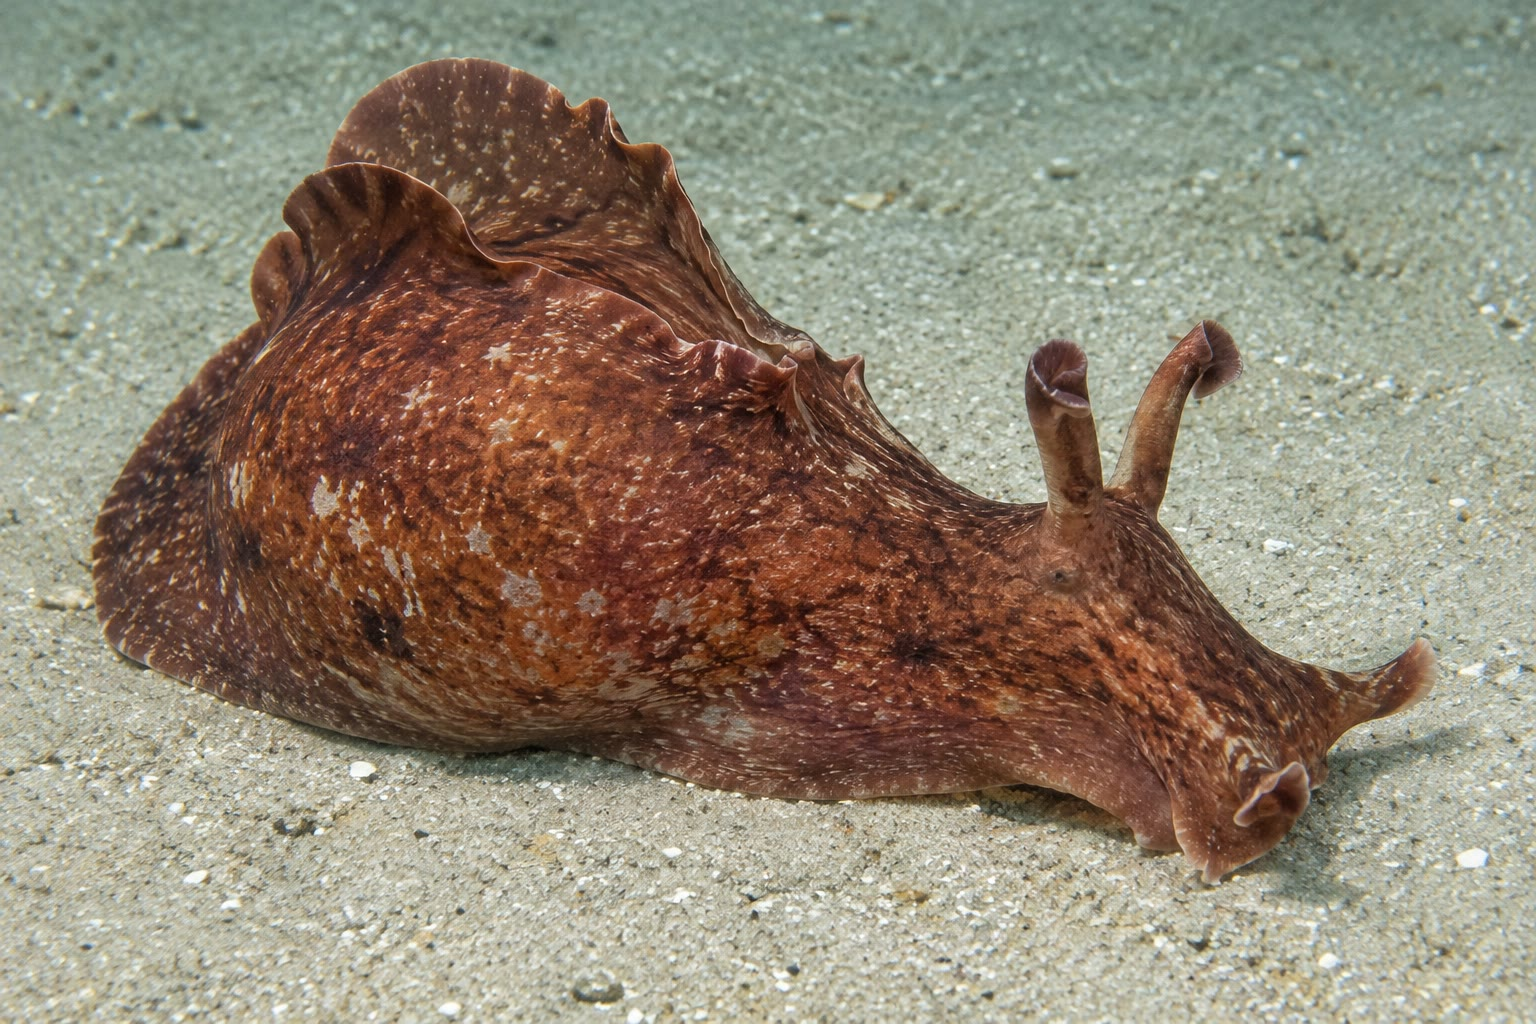
\includegraphics[width=0.46\linewidth]{images/book5/ai/b5-19-aplysia.jpg}\hspace{0.04\linewidth}
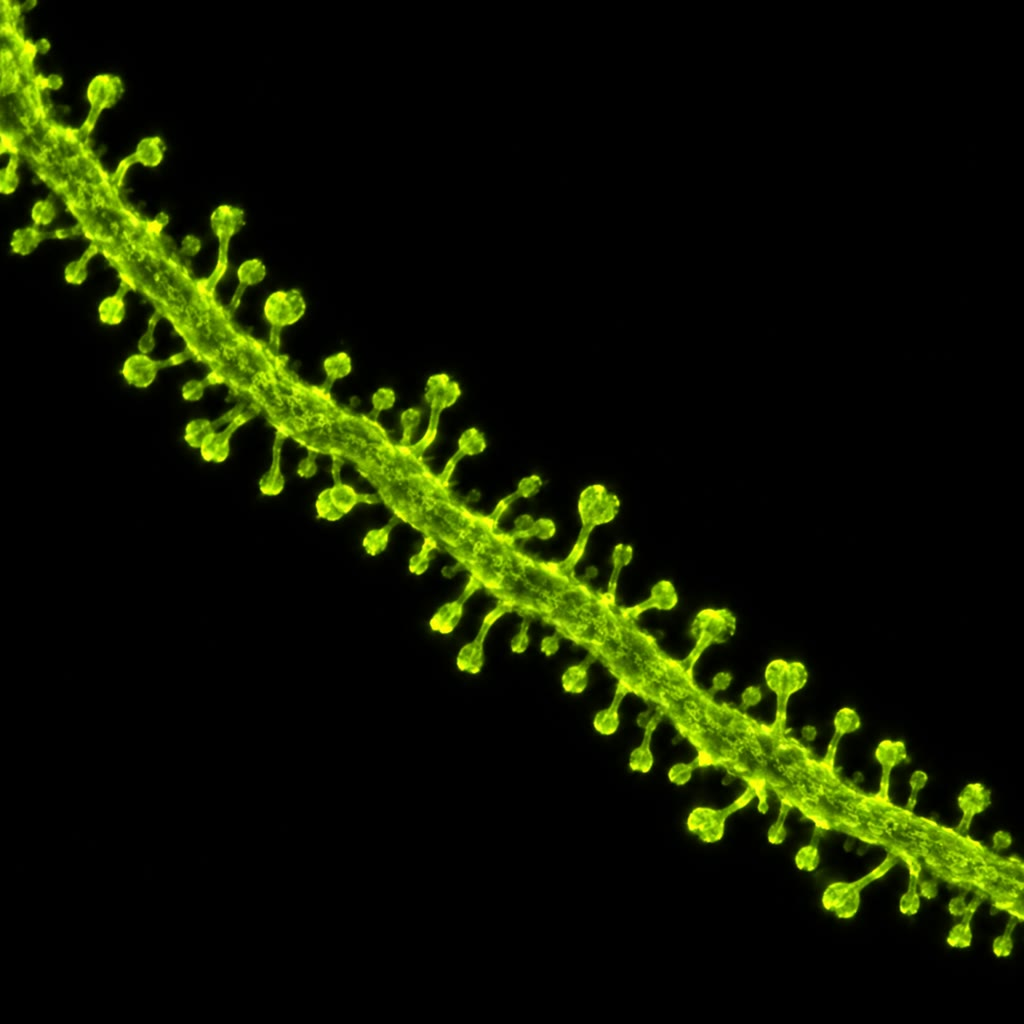
\includegraphics[width=0.36\linewidth]{images/book5/ai/b5-19-dendritic-spines.jpg}

{\small À esquerda: \emph{Aplysia californica}, cujos neurônios, poucos
e grandes, permitem encontrar e registrar a sinapse de uma memória. À
direita: um dendrito cravejado de espinhas, cada uma o lado
pós-sináptico de uma sinapse excitatória e cada uma um compartimento
cujo cálcio decide seu próprio destino.}
\end{omfigure}

\section{Circuitos para lugares e acontecimentos}

\begin{definition}[O circuito hipocampal]\label{def:b3:learning-memory:hippocampus}
\index{giro denteado}\index{CA3}\index{CA1}\index{célula de lugar}\index{célula de grade}\index{completamento de padrões}\index{reativação}
A entrada cortical chega ao \omterm{def:b3:learning-memory:kinds}{hipocampo} pelo córtex entorrinal e passa por
três estágios: o \emph{giro denteado}, cujas células granulares
excedem em número suas entradas e disparam de modo esparso (separando
padrões parecidos); a \emph{CA3}, cujas células piramidais se conectam
recorrentemente entre si, cada uma recebendo milhares de sinapses de
outras --- uma rede \emph{autoassociativa} capaz de completar um padrão
armazenado a partir de um fragmento; e a \emph{CA1}, que compara a saída
da CA3 com a entrada direta e devolve o resultado ao córtex. Num rato
que explora uma arena, uma célula piramidal do \omterm{def:b3:learning-memory:kinds}{hipocampo} dispara apenas
quando o animal está num lugar --- uma \emph{célula de lugar} (O'Keefe,
1971) --- e algumas centenas delas mapeiam a arena; no córtex entorrinal
a montante, as \emph{células de grade} (Moser, 2005) disparam nos
vértices de uma malha hexagonal que cobre o espaço, um sistema de
coordenadas a partir do qual os campos de lugar são construídos. Durante
o sono e o repouso as sequências de células de lugar que dispararam
durante um percurso são \emph{reativadas} em alta velocidade, e bloquear
essa reativação prejudica a memória do percurso: o \omterm{def:b3:learning-memory:kinds}{hipocampo} ensaia ao
córtex os caminhos do dia.
\end{definition}

\begin{omfigure}
\begin{tikzpicture}[every node/.style={font=\scriptsize}, >=stealth]
  % trisynaptic loop
  \node[draw, thick, rounded corners, fill=gray!15, align=center] (ec) at (0,0) {córtex entorrinal\\(células de grade)};
  \node[draw, thick, rounded corners, fill=omDef!20, align=center] (dg) at (3.2,1.4) {giro denteado:\\separação de padrões};
  \node[draw, thick, rounded corners, fill=omProp!30, align=center] (ca3) at (7.2,1.4) {CA3, recorrente:\\completamento de padrões};
  \node[draw, thick, rounded corners, fill=omMeth!25, align=center] (ca1) at (7.2,-1.4) {CA1:\\compara, emite};
  \draw[->, thick] (ec) -- (dg); \draw[->, thick] (dg) -- (ca3); \draw[->, thick] (ca3) -- (ca1); \draw[->, thick] (ca1) -- (ec) node[pos=0.3, below, sloped, font=\tiny] {de volta ao córtex};
  \draw[->, thick, dashed] (ec) -- (ca1.north west) node[pos=0.7, above, sloped, font=\tiny] {via direta};
  \draw[->, thick, omProp!80!black] (ca3.north) .. controls (6.6,2.6) and (7.8,2.6) .. (ca3.north east) node[pos=0.5, above, font=\tiny] {colaterais recorrentes};
  % place field map
  \begin{scope}[xshift=10.4cm, yshift=-0.2cm]
    \draw[thick] (0,0) rectangle (3,2.4); \node[below] at (1.5,-0.05) {a arena, vista de cima};
    \foreach \p/\c in {(0.7,1.8)/omThm, (2.1,1.9)/omDef, (1.4,0.9)/omMeth, (2.5,0.6)/omProp} { \fill[\c!60] \p circle (0.32); \fill[\c!90] \p circle (0.16); }
    \node[above] at (1.5,2.45) {campos de disparo de quatro células de lugar};
  \end{scope}
\end{tikzpicture}

{\small À esquerda: a alça hipocampal --- separação no \omterm{def:b3:learning-memory:hippocampus}{giro denteado},
armazenamento e completamento na \omterm{def:b3:learning-memory:hippocampus}{CA3} recorrente, comparação na \omterm{def:b3:learning-memory:hippocampus}{CA1}. À
direita: cada \omterm{def:b3:learning-memory:hippocampus}{célula de lugar} dispara numa região da arena; juntas, elas
mapeiam o espaço.}
\end{omfigure}

\begin{proposition}[Quanto guarda uma rede autoassociativa]\label{prop:b3:learning-memory:capacity}
\index{rede de Hopfield}\index{capacidade de memória}
Uma rede de $N$ neurônios, cada um conectado a todos os outros com pesos
hebbianos $w_{ij} \propto \sum_{\mu}\xi_{i}^{\mu}\xi_{j}^{\mu}$ somados
sobre os padrões binários armazenados $\xi^{\mu}$, recupera um padrão
armazenado a partir de uma pista corrompida ou parcial acomodando-se
nele como num atrator (Hopfield, 1982). Ela o faz de modo confiável para
até cerca de $P
\approx 0.14N$ padrões aleatórios; além disso os padrões
interferem e a recuperação desmorona. A \omterm{def:b3:learning-memory:hippocampus}{CA3} de um rato, com uns
$3\times 10^{5}$ células piramidais, poderia por essa estimativa guardar
uns $4\times 10^{4}$ padrões --- a ordem dos lugares ou episódios
distintos que um animal encontra numa estação --- e seu disparo esparso
(alguns por cento das células ativas em qualquer padrão) eleva mais
ainda a capacidade. O \omterm{def:b3:learning-memory:hippocampus}{completamento de padrões} a partir de uma pista é o
que permite que um cheiro ou uma esquina evoquem uma cena inteira; o
preço é que memórias parecidas se fundem, o que a separação do \omterm{def:b3:learning-memory:hippocampus}{giro
denteado} combate.
\end{proposition}
\admitted

\begin{method}[Testar a memória e seu mecanismo]\label{met:b3:learning-memory:tests}
\index{labirinto aquático de Morris}\index{condicionamento de medo}\index{engrama}
(1) Uma tarefa espacial: o \omterm{met:b3:learning-memory:tests}{labirinto aquático de Morris} --- um rato nada
em água opaca até uma plataforma escondida num lugar fixo, aprende sua
posição pelas pistas da sala ao longo de dias, e é testado pelo tempo
que passa procurando no quadrante certo quando a plataforma é retirada;
lesões do \omterm{def:b3:learning-memory:kinds}{hipocampo}, bloqueadores de NMDA e a perda da LTP abolem, cada
um, o aprendizado. (2) Uma tarefa associativa: o \omterm{met:b3:learning-memory:tests}{condicionamento de medo}
--- um tom pareado com um choque na pata passa a provocar imobilidade; a
memória depende da amígdala, e uma versão específica de contexto, do
\omterm{def:b3:learning-memory:kinds}{hipocampo}. (3) Um teste de mecanismo: bloqueie o candidato (um fármaco,
um \omterm{def:b3:genetic-engineering:transgenic}{nocaute} restrito a uma região e a um tempo) e mostre que o
aprendizado falha enquanto a percepção e o movimento não. (4) O
engrama: marque os neurônios ativos durante o aprendizado com um canal
sensível à luz (\cref{ch:b3:nervous-systems}) e depois reative-os com
luz --- o animal se imobiliza num contexto seguro, como se se lembrasse;
silenciá-los bloqueia a evocação. A memória está em células
identificáveis e em suas sinapses, e pode ser ligada e desligada.
\end{method}

\begin{omfigure}
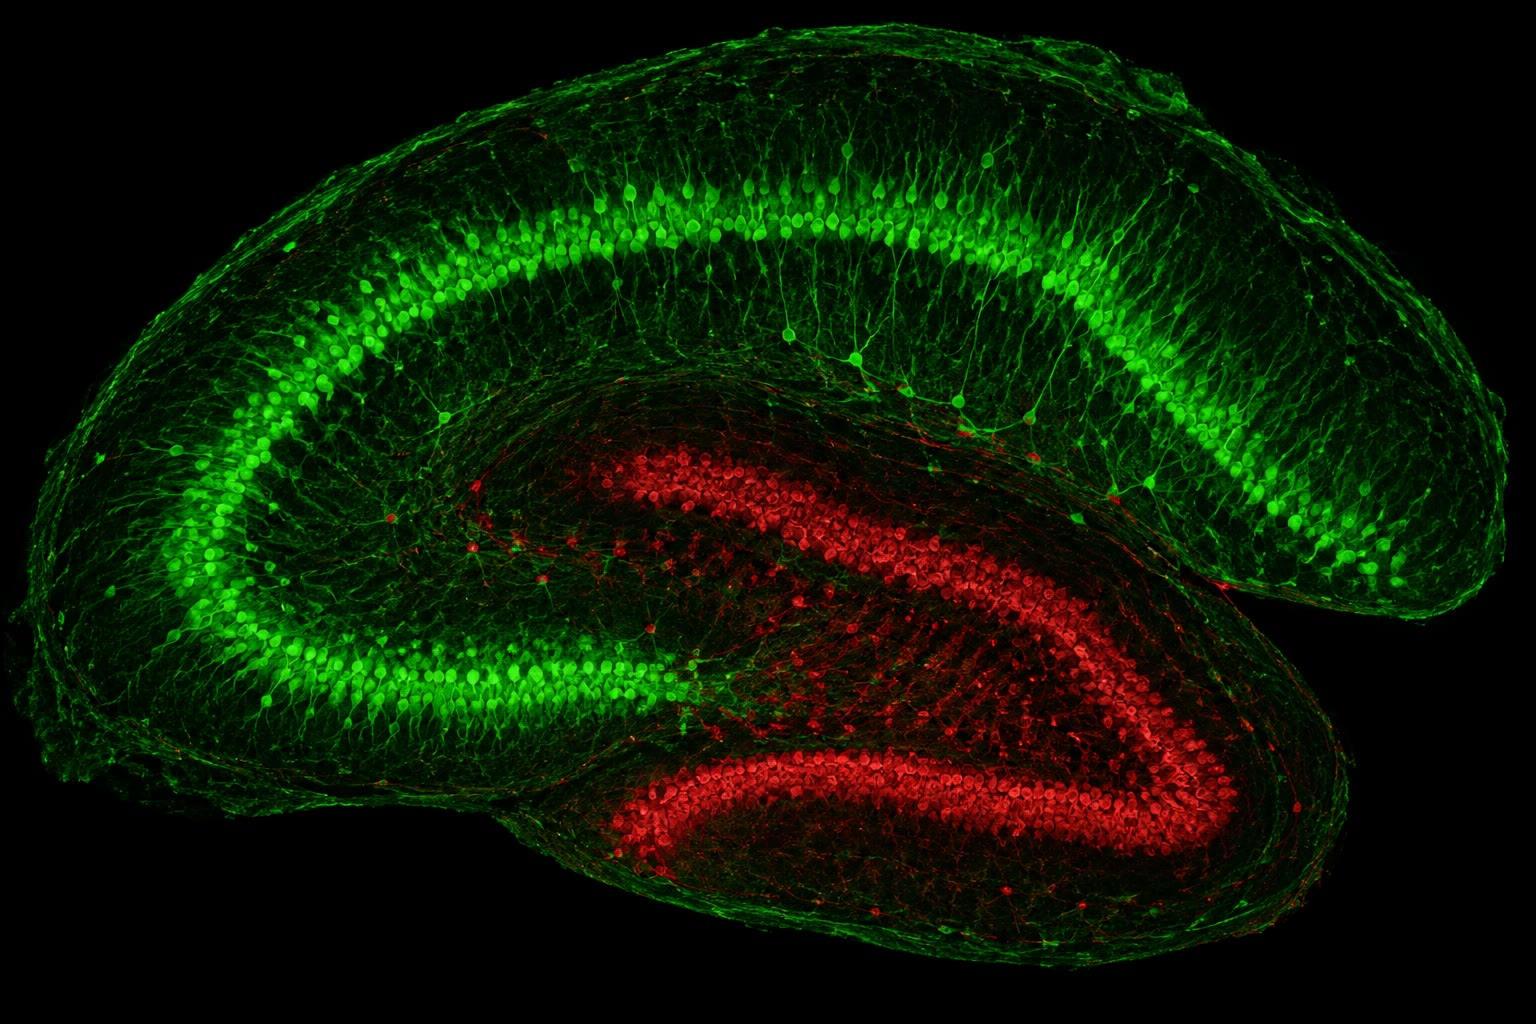
\includegraphics[width=0.56\linewidth]{images/book5/ai/b5-19-hippocampus-section.jpg}

{\small Um corte do \omterm{def:b3:learning-memory:kinds}{hipocampo} de roedor: a faixa curva de células
piramidais (verde) da \omterm{def:b3:learning-memory:hippocampus}{CA3} à \omterm{def:b3:learning-memory:hippocampus}{CA1} e o \omterm{def:b3:learning-memory:hippocampus}{giro denteado} entrelaçado
(vermelho). Toda memória espacial do animal passa por essa alça.}
\end{omfigure}

\section{Recompensa, predição e a plasticidade de uma vida}

\begin{proposition}[Aprender por erro de predição]\label{prop:b3:learning-memory:rescorla}
\index{regra de Rescorla--Wagner}\index{erro de predição}\index{dopamina}
Seja $V$ o valor que um animal atribui a uma pista e $\lambda$ a
recompensa que a segue. A regra de Rescorla--Wagner (1972) diz que a
cada tentativa o valor muda por uma fração $\alpha$ do \emph{\omterm{prop:b3:learning-memory:rescorla}{erro de
predição}}:
\[
\Delta V = \alpha\,(\lambda - V), \qquad
V_{n} = \lambda\bigl(1 - (1-\alpha)^{n}\bigr) ,
\]
de modo que o aprendizado é rápido no início e desacelera à medida que a
predição melhora, para quando a recompensa é plenamente prevista e se
inverte (extinção) quando a recompensa é retirada. Quando duas pistas
são apresentadas juntas elas compartilham uma predição, de modo que uma
pista que nada acrescenta a uma predição já feita não é aprendida (o
\emph{bloqueio}). Schultz (1997) registrou neurônios dopaminérgicos do
mesencéfalo de macacos e verificou que eles disparam a uma recompensa
inesperada, silenciam a uma plenamente prevista e caem abaixo da linha
de base quando uma recompensa prevista não chega: eles transmitem
$\lambda - V$, o próprio \omterm{prop:b3:learning-memory:rescorla}{erro de predição}, ao estriado e ao córtex, onde
a dopamina libera a plasticidade nas sinapses que estiveram ativas há
pouco. Aprender o que prevê recompensa é plasticidade hebbiana com um
terceiro fator que diz se o desfecho foi melhor ou pior que o esperado
--- e as drogas de abuso, ao acionarem a dopamina diretamente,
falsificam um permanente ``melhor que o esperado''.
\end{proposition}
\begin{proof}
A recorrência $V_{n+1} = V_{n} + \alpha(\lambda - V_{n})$ dá $\lambda - V_{n+1} = (1-\alpha)(\lambda - V_{n})$, de modo que o erro encolhe
geometricamente, $\lambda - V_{n} = (1-\alpha)^{n}\lambda$ a partir de
$V_{0} =
0$, donde a fórmula. Para duas pistas $A$ e $B$ apresentadas
juntas a predição é $V_{A} + V_{B}$; se $A$ foi treinada primeiro até
$V_{A} = \lambda$, o erro nas tentativas compostas é zero e $B$ nada
adquire.
\end{proof}

\begin{omfigure}
\begin{tikzpicture}
\begin{axis}[
  width=6.6cm, height=5.0cm,
  axis x line=bottom, axis y line=left,
  xmin=0, xmax=25, ymin=0, ymax=1.1,
  xlabel={tentativa $n$}, ylabel={$V_{n}/\lambda$},
  xlabel style={font=\small, at={(axis description cs:0.5,-0.14)}, anchor=north}, ylabel style={font=\small},
  tick label style={font=\scriptsize}, xtick={0,5,10,15,20,25}, ytick={0,0.5,1},
  clip=false,
]
\addplot[very thick, omDef, domain=0:12, samples=13] {1-0.8^x};
\addplot[very thick, omDef, domain=12:25, samples=14] {(1-0.8^12)*0.8^(x-12)};
\draw[dashed, gray] (axis cs:12,0) -- (axis cs:12,1.05);
\node[font=\scriptsize, anchor=north west, align=left] at (axis cs:0.5,0.98) {recompensa dada:\\aquisição};
\node[font=\scriptsize, anchor=north west, align=left] at (axis cs:14,0.98) {recompensa retirada:\\extinção};
\end{axis}
\begin{axis}[
  at={(7.6cm,0)}, anchor=south west,
  width=6.6cm, height=5.0cm,
  ybar, bar width=14pt,
  axis x line=bottom, axis y line=left,
  ymin=-1.2, ymax=1.5,
  symbolic x coords={unexpected reward, predicted reward, reward omitted},
  xtick=data, xticklabels={recompensa inesperada, recompensa prevista, recompensa omitida}, ytick={-1,0,1}, yticklabels={queda,linha de base,salva},
  ylabel={disparo dopaminérgico},
  x tick label style={font=\scriptsize, align=center, text width=1.9cm}, ylabel style={font=\small}, tick label style={font=\scriptsize},
  clip=false,
]
\addplot[fill=omThm!50, draw=omThm] coordinates {(unexpected reward,1.2) (predicted reward,0.05) (reward omitted,-1.0)};
\end{axis}
\end{tikzpicture}

{\small À esquerda: a curva de aprendizado de Rescorla--Wagner com
$\alpha = 0.2$ --- aproximação geométrica do valor da recompensa, e
depois a extinção quando a recompensa cessa. À direita: os neurônios
dopaminérgicos relatam o \omterm{prop:b3:learning-memory:rescorla}{erro de predição} --- uma salva para a surpresa,
nada para uma recompensa prevista, uma queda quando uma recompensa
prevista falha.}
\end{omfigure}

\begin{definition}[Períodos críticos e as doenças da plasticidade]\label{def:b3:learning-memory:critical}
\index{período crítico}\index{dominância ocular}\index{dependência química}\index{doença de Alzheimer}
A plasticidade é maior em janelas do desenvolvimento. Hubel e Wiesel (na
década de 1960) taparam um olho de um gatinho por algumas semanas após o
nascimento: o córtex visual, normalmente acionado pelos dois olhos em
colunas alternadas, passou a ser acionado quase inteiramente pelo olho
aberto, e o olho privado ficou funcionalmente cego pelo resto da vida
--- ao passo que a mesma privação num gato adulto nada mudava. Esses
\emph{períodos críticos}, para a visão, para a linguagem, para os cantos
das aves, se fecham quando os circuitos inibitórios amadurecem e a
matriz extracelular enrijece, e podem ser reabertos um pouco por
fármacos e treino. As patologias da plasticidade são de dose e de alvo:
a \emph{dependência química} é aprendizado movido por um \omterm{prop:b3:learning-memory:rescorla}{erro de
predição} falsificado, que constrói hábitos que sobrevivem ao prazer; o
transtorno de estresse pós-traumático é uma memória de medo
superconsolidada por hormônios do estresse; e a \emph{doença de
Alzheimer} começa onde a \omterm{def:b3:learning-memory:kinds}{memória declarativa} começa, no córtex
entorrinal e no \omterm{def:b3:learning-memory:kinds}{hipocampo}, com a perda de sinapses --- que acompanha a
demência melhor que qualquer contagem de placas --- antes da perda de
neurônios.
\end{definition}

\begin{remark}[Do que a memória é feita]\label{rem:b3:learning-memory:what}
Uma memória não é uma gravação, mas uma mudança nas forças e nos números
das sinapses, distribuída pelas células que estavam ativas quando ela
foi feita, registrada por uma regra que fortalece o que dispara junto,
liberada por um sinal que diz se o desfecho importou, e ensaiada no sono
até que o córtex a guarde sozinho. A regra é a de Hebb, a porta é o
\omterm{prop:b3:learning-memory:nmda}{receptor NMDA}, o sinal é a dopamina, o ensaio é a \omterm{def:b3:learning-memory:hippocampus}{reativação}, e a
matemática diz quanto um sistema desses pode guardar e por que ele
confunde o que é parecido. Todo experimento que ligou ou desligou uma
memória --- por um bloqueador, um gene, uma luz --- a encontrou nessas
sinapses, nessas células. H.M. morreu em 2008; seu encéfalo, cortado e
fotografado, mostrou a lesão que havia ensinado o campo, e nada mais.
\end{remark}

\section{Exercícios}

\begin{exercise}[$\star$]\label{exo:b3:learning-memory:1}
Distinga a \omterm{def:b3:learning-memory:kinds}{memória declarativa} da não declarativa pelo desempenho de
H.M., e nomeie uma região encefálica para cada um de quatro tipos de
memória não declarativa.
\end{exercise}

\begin{exercise}[$\star$]\label{exo:b3:learning-memory:2}
Enuncie o postulado de Hebb e as três propriedades da LTP que dele
decorrem.
\end{exercise}

\begin{exercise}[$\star$]\label{exo:b3:learning-memory:3}
Explique por que o \omterm{prop:b3:learning-memory:nmda}{receptor NMDA} é um detector de coincidências e o que
acontece com a LTP quando seu bloqueador AP5 é aplicado antes e depois
do tétano.
\end{exercise}

\begin{exercise}[$\star$]\label{exo:b3:learning-memory:4}
Na \emph{Aplysia}, o que distingue a \omterm{def:b3:learning-memory:kinds}{sensibilização} de curto prazo da de
longo prazo no nível molecular, e que experimento o mostra?
\end{exercise}

\begin{exercise}[$\star\star$]\label{exo:b3:learning-memory:5}
Com $\alpha = 0.3$, quantas tentativas até $V$ alcançar \qty{90}{\%} de
$\lambda$? Se a recompensa for então retirada, quantas tentativas até
$V$ cair abaixo de \qty{10}{\%}? Por que a aquisição e a extinção são
simétricas neste modelo, e são simétricas nos animais?
\end{exercise}

\begin{exercise}[$\star\star$]\label{exo:b3:learning-memory:6}
Duas entradas têm $C = \begin{pmatrix}1 & 0.5\\ 0.5 & 1\end{pmatrix}$.
Encontre os autovetores e os autovalores, e diga para que direção a
\omterm{def:b3:learning-memory:ltp}{regra de Hebb} gira os pesos e o que o neurônio então detecta. Aplique a
regra de Oja por um passo a partir de $\mathbf{w} = (1,0)$ com entrada
$\mathbf{x}
= (1,1)$ e $\eta = 0.1$.
\end{exercise}

\begin{exercise}[$\star\star$]\label{exo:b3:learning-memory:7}
Uma espinha tem volume de \qty{0.1}{fL}. A entrada de $500$ íons de
cálcio eleva sua concentração livre em quanto (em
$\unit{\micro mol/L}$), se \qty{95}{\%} são imediatamente ligados por
tampões? Compare com o valor de repouso de \qty{0.1}{\micro mol/L} e com
o $K_{d}$ da calmodulina, ativadora da CaMKII, de cerca de
\qty{1}{\micro mol/L}.
\end{exercise}

\begin{exercise}[$\star\star$]\label{exo:b3:learning-memory:8}
Explique o bloqueio com a regra de Rescorla--Wagner e dê o registro
dopaminérgico correspondente a cada etapa.
\end{exercise}

\begin{exercise}[$\star\star$]\label{exo:b3:learning-memory:9}
Preveja os resultados de (a) deleção do \omterm{prop:b3:learning-memory:nmda}{receptor NMDA} restrita à \omterm{def:b3:learning-memory:hippocampus}{CA1},
(b) um inibidor da síntese proteica dado durante o treino, (c) o mesmo
inibidor dado um dia depois, (d) \omterm{def:b3:learning-memory:hippocampus}{reativação} optogenética das células do
\omterm{def:b3:learning-memory:hippocampus}{giro denteado} que estavam ativas durante um \omterm{met:b3:learning-memory:tests}{condicionamento de medo}, num
contexto novo.
\end{exercise}

\begin{exercise}[$\star\star\star$]\label{exo:b3:learning-memory:10}
Mostre que, só com a \omterm{def:b3:learning-memory:ltp}{regra de Hebb}, o comprimento de $\mathbf{w}$ cresce
sem limite, e que a regra de Oja tem $|\mathbf{w}| = 1$ em qualquer ponto
fixo. Por que o crescimento ilimitado é um problema biológico, e que
mecanismos (escalonamento sináptico, LTD, sono) poderiam corresponder ao
termo normalizador?
\end{exercise}

\begin{exercise}[$\star\star\star$]\label{exo:b3:learning-memory:11}
A \omterm{def:b3:learning-memory:hippocampus}{CA3} de um rato tem $3\times 10^{5}$ células; a de um humano, cerca de
$2\times 10^{6}$. Estime a capacidade de Hopfield de cada uma. Por que a
estimativa é uma medida ruim de quantas memórias uma pessoa guarda, e o
que o papel do \omterm{def:b3:learning-memory:kinds}{hipocampo} na \omterm{def:b3:learning-memory:kinds}{consolidação} acrescenta ao quadro?
\end{exercise}

\begin{exercise}[$\star\star\star$]\label{exo:b3:learning-memory:12}
Gatinhos privados da visão de um olho por semanas perdem o território
cortical desse olho; adultos não. Explique, pela competição hebbiana,
por que o olho aberto vence, por que a privação binocular tem efeito
menor que a monocular, e o que fecha o \omterm{def:b3:learning-memory:critical}{período crítico}.
\end{exercise}

\section{Problema: Uma Sinapse Que Lembra}

\begin{problem}[{Problema de fim de semana --- uma memória seguida do
cálcio numa espinha até um rato num labirinto: a aritmética de cálcio da
indução, um neurônio hebbiano convergindo para o que suas entradas têm
em comum, uma curva de aprendizado cronometrada pelo erro de predição e
a capacidade de um hipocampo, terminando na concentração de cálcio que
induz a LTP, nas tentativas de que um rato precisa e nos padrões que sua
CA3 consegue guardar}]
\label{pb:b3:learning-memory:1}
Dados: uma espinha de volume \qty{0.08}{fL}; cada canal NMDA conduz
$10^{3}$ Ca$^{2+}$ por abertura de \qty{50}{ms}; uma sinapse tem $10$
\omterm{prop:b3:learning-memory:nmda}{receptores NMDA}; \qty{98}{\%} do cálcio que entra é tamponado; cálcio
livre de repouso de \qty{0.1}{\micro mol/L}; a CaMKII é ativada acima de
\qty{2}{\micro mol/L} de cálcio livre, e a calcineurina entre $0.3$ e
\qty{1}{\micro mol/L}. Hebb: duas entradas com $C = \begin{pmatrix}1 &
0.6\\ 0.6 & 1\end{pmatrix}$, $\eta = 0.1$. Rescorla--Wagner: $\alpha =
0.15$. Capacidade: \omterm{def:b3:learning-memory:hippocampus}{CA3} de rato com $3\times 10^{5}$ células, $P = 0.14N$; um rato explora $20$ lugares novos por dia.

\medskip
\noindent\textbf{Parte I --- Cálcio.}
\begin{enumerate}
  \item Os dez \omterm{prop:b3:learning-memory:nmda}{receptores NMDA} abrem uma vez. Quantos íons de cálcio
        entram, quantos ficam livres, e que elevação de concentração é
        essa na espinha?
  \item A CaMKII é ativada? E se apenas dois receptores abrirem
        (glutamato liberado, mas a espinha mal despolarizada)?
  \item Com dois receptores abertos, que enzima está em sua faixa, e o
        que acontece com a sinapse? Explique como um mesmo íon pode
        produzir tanto LTP quanto LTD.
  \item O cálcio é bombeado para fora com constante de tempo de
        \qty{20}{ms}. Por que as entradas precisam chegar dentro de
        dezenas de milissegundos para somar seu cálcio, e como isso fixa
        a janela de tempo de disparo?
  \item Uma espinha está a \qty{0.5}{\micro m} de sua vizinha no
        dendrito. Explique por que o tamponamento e o pescoço estreito
        da espinha mantêm o sinal de cálcio numa só espinha, e por que
        isso importa para a especificidade de entrada.
  \item O bloqueio por magnésio é aliviado por volta de \qty{-30}{mV}.
        Uma única sinapse AMPA despolariza a espinha em \qty{5}{mV} a
        partir de \qty{-70}{mV}. Quantas entradas sincrônicas (ou o que
        mais) são necessárias para desbloquear os \omterm{prop:b3:learning-memory:nmda}{receptores NMDA}? O que
        isso diz sobre a \omterm{def:b3:structural-biology:allostery}{cooperatividade}?
\end{enumerate}

\medskip
\noindent\textbf{Parte II --- Um neurônio hebbiano.}
\begin{enumerate}[resume]
  \item Encontre os autovalores e autovetores de $C$.
  \item Partindo de $\mathbf{w} = (1, 0)$, aplique a \omterm{def:b3:learning-memory:ltp}{regra de Hebb} média
        $\mathbf{w} \leftarrow \mathbf{w} + \eta C\mathbf{w}$ por três
        passos. Qual é o ângulo de $\mathbf{w}$ com a direção $(1,1)$
        após cada um?
  \item Depois de muitos passos, qual é a razão $w_{2}/w_{1}$, e o que
        acontece com $|\mathbf{w}|$?
  \item Aplique a regra de Oja média $\mathbf{w} \leftarrow \mathbf{w} +
        \eta\,(C\mathbf{w} - (\mathbf{w}^{\mathsf{T}}C\mathbf{w})
        \mathbf{w})$ por um passo a partir de $(0.8, 0.8)$. Para onde
        ela se move?
  \item O neurônio agora responde às duas entradas juntas. Se a entrada
        2 disparar sozinha (algo raro), quanto vale $y$ em relação ao
        caso conjunto, com $\mathbf{w} = (0.71, 0.71)$?
  \item Explique numa frase como a associatividade da LTP (uma entrada
        fraca pareada com uma forte é fortalecida) é este teorema em
        ação.
\end{enumerate}

\medskip
\noindent\textbf{Parte III --- Curva de aprendizado.}
\begin{enumerate}[resume]
  \item Com $\alpha = 0.15$, calcule $V_{n}/\lambda$ após $5$, $10$ e
        $20$ tentativas.
  \item Quantas tentativas para alcançar \qty{95}{\%} de $\lambda$?
  \item Um rato aprende um labirinto em cerca desse número de
        tentativas. Se a recompensa for dobrada, o modelo prevê
        aprendizado mais rápido em tentativas? O que muda?
  \item A pista A é treinada até a assíntota; depois A e B são
        apresentadas juntas com a mesma recompensa por $20$ tentativas.
        Quanto vale $V_{B}$? O que fazem os neurônios dopaminérgicos nas
        tentativas compostas?
  \item A recompensa agora segue B sozinha. Descreva o \omterm{prop:b3:learning-memory:rescorla}{erro de predição}
        e a resposta dopaminérgica da primeira tentativa, e o curso de
        $V_{B}$.
  \item Um fármaco eleva a dopamina independentemente do desfecho. Usando
        a regra, explique por que as ações que precedem o fármaco são
        aprendidas como se tivessem sido recompensadas, quaisquer que
        sejam suas consequências.
\end{enumerate}

\medskip
\noindent\textbf{Parte IV --- O \omterm{def:b3:learning-memory:kinds}{hipocampo}.}
\begin{enumerate}[resume]
  \item Capacidade de Hopfield da \omterm{def:b3:learning-memory:hippocampus}{CA3} do rato.
  \item A $20$ lugares novos por dia, quanto tempo até a capacidade ser
        atingida? O que precisa acontecer para o animal continuar
        aprendendo?
  \item A \omterm{def:b3:learning-memory:kinds}{consolidação} transfere memórias ao córtex ao longo de semanas.
        Explique por que uma transferência lenta protege as memórias
        corticais antigas (interferência catastrófica) e por que o
        \omterm{def:b3:learning-memory:kinds}{hipocampo} é um depósito temporário.
  \item Se \qty{3}{\%} das células da \omterm{def:b3:learning-memory:hippocampus}{CA3} estão ativas em qualquer
        padrão, quantas células codificam um lugar, e quantos padrões
        poderiam ser distinguidos se se exigisse que os padrões
        compartilhassem menos da metade de suas células? (Argumente
        qualitativamente por que a codificação esparsa eleva a
        capacidade.)
  \item A \omterm{def:b3:learning-memory:hippocampus}{reativação} durante o sono comprime um percurso de \qty{10}{s}
        em \qty{0.5}{s}. Se a janela de tempo de disparo é de
        \qty{20}{ms}, que separação entre os disparos das \omterm{def:b3:learning-memory:hippocampus}{células de
        lugar} no percurso se torna hebbiana na \omterm{def:b3:learning-memory:hippocampus}{reativação}? Por que essa
        pode ser a razão de ser da compressão?
  \item A memória do labirinto sobrevive a uma lesão do \omterm{def:b3:learning-memory:kinds}{hipocampo} feita
        um mês depois do treino, mas não a uma feita um dia depois.
        Interprete, com o padrão de perda de H.M.
  \item Resuma: a concentração de cálcio livre após dez aberturas de
        NMDA (questão~1), as tentativas até \qty{95}{\%} de aprendizado
        (questão~14) e a capacidade da \omterm{def:b3:learning-memory:hippocampus}{CA3} do rato (questão~19).
\end{enumerate}
\end{problem}
